\documentclass[12pt, a4paper]{book}

\usepackage{fancyhdr}
\usepackage[left=4cm, right=4cm, top=4cm, bottom=4cm]{geometry}
\usepackage[utf8]{inputenc}
\usepackage[table]{xcolor}
\usepackage{hyperref}
\usepackage{amsmath}
\usepackage{enumitem}
\usepackage[linewidth=1pt]{mdframed}
\usepackage{graphicx}
\usepackage{amsfonts}
\usepackage{centernot}
\usepackage{booktabs}
\usepackage{subcaption}
\usepackage[justification=centering]{caption}

\DeclareMathOperator*{\argmax}{argmax}
\DeclareMathOperator*{\argmin}{argmin}
\newcolumntype{L}{>{$}l<{$}} % math-mode version of "l" column type

\newcommand{\coursetitle}{Statistical Machine Learning}
\newcommand{\doctitle}{Homework2}
\newcommand{\name}{Mohammadreza Ghofrani}
\newcommand{\studentno}{400131076}
\newcommand{\todaydate}{\today}

% \settextfont{XB Kayhan}
% \setlatintextfont{Times Newer Roman}

\pagestyle{fancy}
\lhead{\name}
\rhead{\textbf{\doctitle}}

\begin{document}

\begin{flushright}
    \name \\
    \studentno \\
    \todaydate
\end{flushright}

\vspace*{0.5cm}

\begin{center}
    \huge
    \textbf{\coursetitle}
    \break
    \large
    \doctitle
\end{center}

% suppress the fancy header on the first page only
\thispagestyle{plain}

\section*{Theoretical Problems}

\subsection*{Question One}

We have the definition of empirical distribution function.

\begin{eqnarray*}
    \hat{F_n}(x) = \frac{\sum_{i=1}^n I (X_i \leq x )}{n},
\end{eqnarray*}

where

\begin{eqnarray*}
    I (X_i \leq x) =
    \begin{cases}
        1 & \text{if } X_i \leq x \\
        0 & \text{if } X_i > x
        \end{cases}
\end{eqnarray*}

So to show $\mathbb{E}(\hat{F}_n(x)) = F(x)$, we write as follows:

\begin{align*}
    \mathbb{E}(\hat{F_n}(x)) & = \frac{1}{n} \sum_{i = 1}^n \mathbb{E}(I(X_i \leq x )) \\
     & = \frac{1}{n} \sum_{i = 1}^n \mathbb{P}(X_i \leq x ) \\
     & = \frac{1}{n} \sum_{i = 1}^n F(x) \\
     & = F(x),
\end{align*}

In the prove above we have substitued $\mathbb{E}(I(X_i \leq x))$ with $\mathbb{P}(X_i \leq x)$ based on the
statement ``probability is a special case of expectation" shown in the page 49 of the source book.

Now we will show correctness of $\mathbb{V}(\hat{F}_n(x)) = \frac{F(x)(1-F(x))}{n}$.

\begin{eqnarray*}
    \mathbb{V}(\hat{F_n}(x)) = \mathbb{E}(\hat{F_n}(x)^2) - \mathbb{E}(\hat{F_n}(x))^2
\end{eqnarray*}

Calculating $\mathbb{E}(\hat{F_n}(x)^2)$.

\begin{align*}
    \mathbb{E}(\hat{F_n}(x)^2) & = \frac{1}{n^2} \, \mathbb{E} \big( \sum_{i = 1}^n I(X_i \leq x ) \big)^2 \\
    & = \frac{1}{n^2}  \, \mathbb{E} \Big( \sum_{i = 1}^n I(X_i \leq x )^2 + \sum_{i = 1}^n \sum_{j = 1, j \neq i}^n I(X_i \leq x ) I(X_j \leq x ) \Big) \\
    & = \frac{1}{n^2}  \, \Big( \sum_{i = 1}^n \mathbb{E} ( I(X_i \leq x )^2 ) + \sum_{i = 1}^n \sum_{j = 1, j \neq i}^n \mathbb{E} ( I(X_i \leq x ) I(X_j \leq x ) ) \Big) \\
    & = \frac{1}{n^2}  \, \Big( \sum_{i = 1}^n \mathbb{E} ( I(X_i \leq x ) ) + \sum_{i = 1}^n \sum_{j = 1, j \neq i}^n \mathbb{E} ( I(X_i \leq x ) ) \mathbb{E} ( I(X_j \leq x ) ) \Big) \\
    & = \frac{1}{n^2}  \, \Big( \sum_{i = 1}^n \mathbb{P}(X_i \leq x ) +  \sum_{i = 1}^n \sum_{j = 1, j \neq i}^n \mathbb{P}(X_i \leq x ) \mathbb{P}(X_j \leq x )  \Big) \\
    & = \frac{1}{n^2}  \, \Big( \sum_{i = 1}^n F(x) + \sum_{i = 1}^n \sum_{j = 1, j \neq i}^n F(x)^2  \Big) \\
    & = \frac{1}{n^2}  \, ( nF(x) + (n^2 - n)F(x)^2 ) \\
    & = \frac{1}{n} \, ( F(x) + (n - 1) F(x)^2 )
\end{align*}

Now by plugging in the value of $\mathbb{E}(\hat{F}_n(x)^2)$ we show the correctness of the statement.

\begin{align*}
    \mathbb{V}(\hat{F_n}(x)) & = \frac{1}{n} \, ( F(x) + (n - 1) F(x)^2 ) - F(x)^2 \\
    & = \frac{F(x)(1 - F(x))}{n}
\end{align*}

Correctness of the $\mathbf{M} \mathbf{S} \mathbf{E} $. Based on the theorem 6.9 (page 91) we know
$\mathbf{M} \mathbf{S} \mathbf{E} = \text{bias}^2(\hat{\theta}_n) + \mathbb{V}_\theta(\hat{\theta}_n)$. Thus,

\begin{align*}
    \mathbf{M} \mathbf{S} \mathbf{E} & = \text{bias}^2(F(x)) + \mathbb{V}(F(x)) \\
    & = (\mathbb{E}(\hat{F_n}(x)) - F(x))^2 + \mathbb{V}(F(x)) \\
    & = 0^2 + \mathbb{V}(F(x)) \\
    & = \frac{F(x)(1 - F(x))}{n} \rightarrow 0
\end{align*}

For proving $\hat{F}_n(x) \xrightarrow{P} F(x)$ we use theorem 6.10 in page 91 of the source book.
Based on this theorem if $\text{bias} \rightarrow 0$ and $\text{se} \rightarrow 0$ as $n \rightarrow \infty$
then $\hat{\theta}_n \xrightarrow{P} \theta$. For $\hat{F}_n{(x)}$ we know $\text{bias} = 0$ and for
$\text{se} = \sqrt{\frac{F(x)(1 - F(x))}{n}}$ which limits to zero as $n \rightarrow 0$, so $\hat{F}_n(x) \xrightarrow{P} F(x)$.

\subsection*{Question Two}

Based on the central limit theorem we have $\hat{F}_n(x) \approx N(\mu, \frac{\sigma^2}{n})$. Because
we don't know the exact value of $\mu$ and $\sigma$, we estimate them via $\mathbb{E}(\hat{F}_n(x))$ and
$\mathbb{V}(\hat{F}_n(x))$, respectively, which are calculated in the solution to previous question. Thus,

\begin{align*}
    \hat{F}_n(x) & \approx N( \mu, \frac{\sigma^2}{n}) \\
     & \approx N( F(x), \frac{1}{n} \times \frac{F(x)(1-F(x))}{n}) \\
     & \approx N( F(x), \frac{F(x)(1-F(x))}{n^2})
\end{align*}

as $n \rightarrow \infty$ the expression $\frac{F(x)(1-F(x))}{n^2} \rightarrow 0$. That said,
the distribution of the $\hat{F}_n(x)$ will become a point mass in $F(x)$, which was expected.

\subsection*{Question Three}

\textbf{The momemt estimator}

Using data the first moment is

\begin{align*}
    \hat{\alpha}_1(\theta) = \frac{1}{n} \sum_i X_i
\end{align*}

In other hand we know that $\alpha_1(\theta) = \mathbb{E}(\theta)$. The value of $\mathbb{E}(\theta)$ for
the poisson distribution is $\lambda$. So $\lambda = \frac{1}{n} \sum_i X_i$.

\textbf{The maximum likelihood}

We know that

\begin{align*}
    \mathcal{L}_n(\theta) = \prod_{i=1}^{n} f(x_i; \lambda) = \prod_{i=1}^{n} \lambda^{x_i} \frac{e^{-\lambda}}{x_i!}
\end{align*}

So that the log likelihood will be.

\begin{align*}
    \ell_n(\lambda) = \log \mathcal{L}_n{(\lambda)} = \sum_{i=1}^{n} (x_i\log(\lambda) - \lambda - \log(x_i!))
\end{align*}

by deriving and equating with zero, result would be

\begin{align*}
    \frac{\partial \ell_n(\lambda)}{\partial \lambda} = \sum_{i=1}^{n} (\frac{x_i}{\lambda} - 1) & = 0 \\
    \frac{1}{\lambda} \sum_{i=1}^{n} x_i - n & = 0 \\
    \lambda & = \frac{1}{n} \sum_{i=1}^{n} x_i
\end{align*}

\textbf{Fisher information}

To calculate fisher information, first we need to calculate score function.

\begin{align*}
    s(X;\lambda) = \frac{\partial \log f(X;\lambda)}{\lambda} = \frac{x_i}{\lambda} - 1
\end{align*}

By plugging in the score function into fisher information we will have

\begin{align*}
    I_n(\lambda) & = \sum_{i=1}^{n} \mathbb{V}_\lambda (s(X_i;\lambda)) \\
    & = \sum_{i=1}^{n} \mathbb{V}_\lambda (\frac{x_i}{\lambda} - 1) \\
    & = \sum_{i=1}^{n} \frac{1}{\lambda^2} \mathbb{V}_\lambda(x_i) \\
    & = \sum_{i=1}^{n} \frac{1}{\lambda} \\
    & = \frac{n}{\lambda}
\end{align*}

\subsection*{Question Four}

\subsubsection*{Part a}

The Wald random variable will be calcualted as follows

$$W = \frac{X - n\theta_0}{\sqrt{n\theta_0(1-\theta_0)}} = \frac{60 - 50}{5} = 2$$

Because the dataset is relatively large ($=100$ samples), we can assume that $W$ has standard normal distribution.
Note that our test is one sided meaning that we only want to test whether $P(H) > \frac{1}{2}$ and don't want to check
possiblity of $P(H) < \frac{1}{2}$. So we obtain $z_{0.05} = 1.64$. Comparing the value $z_{0.05}$ with
$W$ ($W > z_{0.05}$) we can say that we can reject $H_0$.

\subsubsection*{Part b}

Here we need to compare the $W$ with $z_{0.01}$ instead of $z_{0.05}$. The value of $W=2$ which has
calucalted in the previous part, but the value of $z_{0.01} = 2.33$. By comparing the value for
$z_{0.01}$ and $W$ ($W < z_{0.01}$) we can't reject $H_0$.

\subsubsection*{Part c}

We find the p-value as follows

\begin{eqnarray*}
    \text{p-value} & = & P(W > c) \\
    & = & P(W > 2) \\
    & = & 1 - \Phi(2) = 0.023
\end{eqnarray*}


\subsection*{Question Five}

First we should mention that $P(X^* = x) = \frac{1}{n}$ for $x=X_1, X_2, ..., X_n$.
By stating this we answering the following parts.

\subsubsection*{Part a}

\begin{align*}
    \mathbb{E}(\overline{X}_n^* | X_1, \dots, X_n) =  \sum_x x P(X^*=x) = \frac{1}{n} \sum_{i=1}^{n} X_i = \overline{X}
\end{align*}

\subsubsection*{Part b}

\begin{align*}
    \mathbb{V}(\overline{X}_n^* | X_1, \dots, X_n) = \sum_x (x - \overline{X})^2 P(X^*=x) = \frac{1}{n^2} \sum_{i=1}^{n} (X_i - \overline{X})^2
\end{align*}

\subsubsection*{Part c}

\begin{align*}
    \mathbb{E}(\overline{X}_n^*) = \mathbb{E}(\mathbb{E}(\overline{X}|X_1, X_2, ..., X_n)) = \mathbb{E}(\overline{X}) = \mu
\end{align*}

\subsubsection*{Part d}

\begin{align*}
    \mathbb{V}(\overline{X}_n^*) & = \mathbb{V}(\mathbb{E}(\overline{X}|X_1, X_2, ..., X_n)) + \mathbb{E}(\mathbb{V}(\overline{X}|X_1, X_2, ..., X_n)) \\
    & = \mathbb{V}(\overline{X}) + \mathbb{E}\bigg(\frac{1}{n^2}\sum_{i=1}^{n} (X_i-\overline{X})^2\bigg) \\
    & = \frac{\sigma^2}{n} + \frac{1}{n^2} \mathbb{E} \bigg( \sum_{i=1}^{n} (X_i - \overline{X})^2 \bigg) \\
    & = \frac{\sigma^2}{n} + \frac{n-1}{n^2} \mathbb{E} \bigg( \frac{\sum_{i=1}^{n} (X_i - \overline{X})^2}{n-1} \bigg) \\
    & = \frac{\sigma^2}{n} + \frac{n-1}{n^2} \sigma^2 \\
    & = \frac{\sigma^2}{n} (2 - \frac{1}{n})
\end{align*}

\clearpage
\section*{Programming Problems}

\subsection*{Question One}

By substituting each of $q$s in the formula $q_1^*=\argmin_q D_{KL}(p||q)$ we come up with
the following results. Based on these results we can say that $q_1^* \sim N(5, 1.5)$.

\begin{mdframed}
    \begin{verbatim}
    q1 ~ N(3, 0.5)
    q2 ~ N(5, 1.5)
    q3 ~ N(7, 0.5)

    D_kl(p||q1)= 7999.2468
    D_kl(p||q2)= 771.4980
    D_kl(p||q3)= 7999.2468
    \end{verbatim}
\end{mdframed}

And for $q_2^*$ where is derived by $q_2^*=\argmax_q D_{KL}(q||p)$ we have the following result.
Based on these results $q_2^*=q_1$ or $q_2^*=q_3$.

\begin{mdframed}
    \begin{verbatim}
    q1 ~ N(3, 0.5)
    q2 ~ N(5, 1.5)
    q3 ~ N(7, 0.5)

    D_kl(q1||p)= -0.0234
    D_kl(q2||p)= 324.8386
    D_kl(q3||p)= -0.0234
    \end{verbatim}
\end{mdframed}

\autoref{pq_star} show the probability density of $p$ relative to each of the $q_i^*$s.
As can be seen here $q_2^*$ has just covered only one peak of $p$. However, $q_1^*$ has tried
to cover both of the peaks. Assuming each of the peaks as one of the images' features,
if we use $q_2^*$ we have images which have only one of the features, but using
$q_1^*$ we will have a mixture of the features. In some cases $q_2^*$ is beneficial
and in the others $q_1^*$. For examples if the features were masculine and feminine attributes,
using $q_1^*$ will generate an image which is not 100\% men nor women. But if the features
were colors using $q_1^*$ will generate a new color which may be appealing in some cases.

\begin{figure}
    \begin{subfigure}{0.45\linewidth}
        \centering
        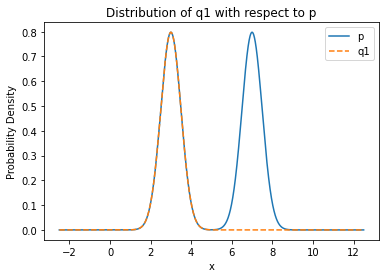
\includegraphics[width=\linewidth]{image/q1/q1p.png}
        \caption{Comparison of probability density between $p$ and $q_2^*=q1$}
    \end{subfigure}
    \hfil
    \begin{subfigure}{0.45\linewidth}
        \centering
        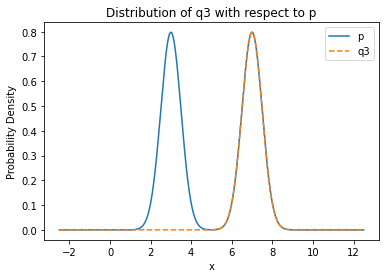
\includegraphics[width=\linewidth]{image/q1/q3p.png}
        \caption{Comparison of probability density between $p$ and $q_2^*=q3$}
    \end{subfigure}
    \newline
    \hspace*{2.5cm}
    \begin{subfigure}{0.5\linewidth}
        \centering
        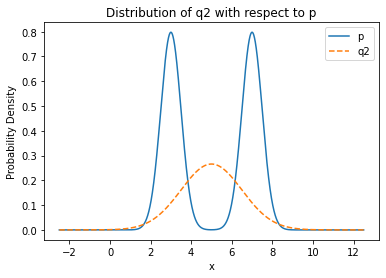
\includegraphics[width=\linewidth]{image/q1/q2p.png}
        \caption{Comparison of probability density between $p$ and $q_1^*=q2$}
    \end{subfigure}
    \caption{Comparison of $p$ with each $q^*$}
    \label{pq_star}
\end{figure}

\subsection*{Question Two}

\subsubsection*{Part a}

Because number of samples are relatively large ($\approx 300$) we can use central limit theorem.
So mean duration is $70.89$ with standard deviation $0.82$.

\subsubsection*{Part b}

Because of the central limit theorem we know the distribution of $\overline{X}$ is nromal. Thus,
using the normal interval method we have

\begin{eqnarray*}
    (\overline{X} - z_5 \times \hat{se}, \overline{X} + z_5 \times \hat{se}) = (69.54, 72.25)
\end{eqnarray*}

\subsubsection*{Part c}

We infer the median from samples, but for the standard deviation we have to use bootstapping method which
results in $\text{median}=76$ and $\hat{se}_{\text{median}} = 0.98$.


\subsection*{Question Three}

\subsubsection*{Part a}

Because the parameters of the distribution are not known, we use the empirical distribuion functions
to find the CDF of the distribution.

\subsubsection*{Part b}

Using the fact stated on the page 99 of the source book, we draw \autoref{q3_cdf}.

\begin{figure}[h]
    \centering
    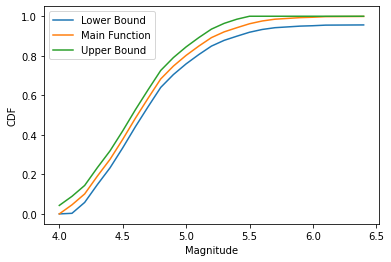
\includegraphics[width=0.5\linewidth]{image/q3/cdf.png}
    \caption{estimated CDF function with its lower and upper bounds}
    \label{q3_cdf}
\end{figure}

\subsubsection*{Part c}

\textbf{Pivotal Method}

In pivotal method we do bootstapping on the available data and create confidence interval based on them.
Confidence interval using this method is $[0.5260, 0.5890]$.

\textbf{Normal Method}

In normal method we assume that the distribution of the target value is normal, so using the standard deviation
of the random variable (for $F$ standard deviation is stated in theorem 7.3) we come up with the
$(0.5262, 0.5878)$

\textbf{Percentile Method}

This method first uses bootstapping to generate samples and estimate a value for $F$. Then reports the
interested percentiles. Confidence interval using this method is $[0.5250, 0.5880]$.

\subsection*{Question Four}

\subsubsection*{Part a}

Using the formula derived in Example 7.13 in page 101 of the source book we have

\begin{eqnarray*}
    \hat{\rho} & = & \frac{\sum_i (X_i - \overline{X}_n)(Y_i - \overline{Y}_n)}{\sqrt{\sum_i (X_i - \overline{X}_n)^2)} \sqrt{\sum_i(Y_i - \overline{Y}_n)^2}} \\
    \hat{\rho} & = & 0.54
\end{eqnarray*}

As we expect all of the three methods result (Pivotal, Normal, Percentile) in the same final interval with little tweaks.

\subsubsection*{Part b}

Using bootstapping method, we iteratively select samples from the given data and re-estimate the value of
correlation coefficient. Standard deviation of these estimated values is the number reported by this method.
Here the value of $\hat{se}_{\hat{p}} = 0.17$.

\subsubsection*{Part c}

\textbf{Pivotal Method}

In pivotal method we do bootstapping on the available data and create confidence interval based on them.
Confidence interval using this method is $[0.20, 0.84]$.

\textbf{Normal Method}

In normal method we assume that the distribution of the target value is normal, so using the standard deviation
of the random variable (for $F$ standard deviation is stated in theorem 7.3) we come up with the
$(16, 0.87)$

\textbf{Percentile Method}

This method first uses bootstapping to generate samples and estimate a value for $F$. Then reports the
interested percentiles. Confidence interval using this method is $[0.24, 0.88]$.

As we expect all of the three methods (Pivotal, Normal, Percentile) result in the same final interval with little tweaks.

\subsection*{Question Five}

\subsubsection*{Part a}

Using Python's numpy library we generate samples from the given distribution.

\subsubsection*{Part b}

Using bootstapping method we come to the following results:

\begin{mdframed}
    \begin{verbatim}
    e_hat: 179.6543
    p_hat_std: 16.2246

    94% Confidence Interval: [152.5282, 212.0277]
    \end{verbatim}
\end{mdframed}

\subsubsection*{Part c}

\autoref{real_bootstapping} shows the difference between sampling from the real distribution and
bootstapping method. Although available data for bootstapping was limited but it could almost show
the real distribution of the estimated random variable, which shows the effectiveness of the
method.

\begin{figure}[h]
    \begin{subfigure}{0.45\linewidth}
        \centering
        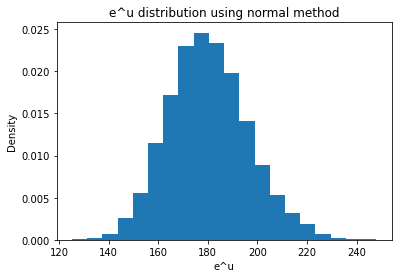
\includegraphics[width=\linewidth]{image/q5/real.png}
        \caption{real}
    \end{subfigure}
    \hfil
    \begin{subfigure}{0.45\linewidth}
        \centering
        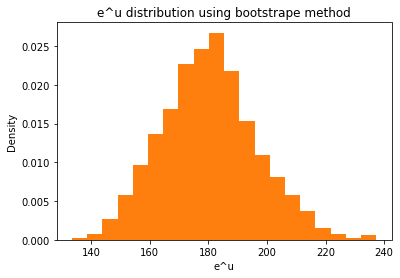
\includegraphics[width=\linewidth]{image/q5/bootstrap.png}
        \caption{bootstap}
    \end{subfigure}
    \caption{Comparison of real sampling histogram versus bootstapping technique}
    \label{real_bootstapping}
\end{figure}

\subsection*{Question Six}

\subsubsection*{Part a}

Using numpy library we generate samples from the given distribution.

\subsubsection*{Part b}

Here is the formula stated in the page 177 of the source book
which we have used to draw the posterior density figure.

$$f(\theta|x) = \frac{f(x|\theta) f(\theta)}{\int f(x|\theta) f(\theta) d\theta}$$

The numinator of the fraction above calculate the value of $f(x|\theta)$ and $f(\theta)$ for a
specific $\theta$. Deminator, on the other hand, calcualtes values of $f(x|\theta)$ and $f(\theta)$
for all values of $\theta$ and sums them up. Using computer simulation we come up with \autoref{q6_posterior_density}.

\begin{figure}[h]
    \centering
    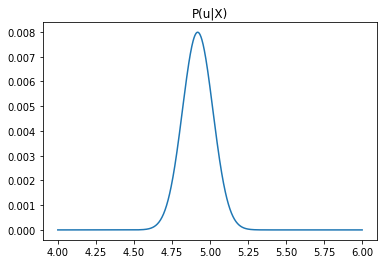
\includegraphics[width=0.5\linewidth]{image/q6/posterior.png}
    \caption{Posterior density of question six}
    \label{q6_posterior_density}
\end{figure}

\subsubsection*{Part c}

\autoref{q6_simulation} shows the histogram of the drawn data.
Comparing the current figure with \autoref{q6_posterior_density}, which shows the true posterior distribution,
we see that the general behavior of both are the same. And as we sample more draws from the posterior distribution,
we have histograms which are closer and closer to original posterior distribution.

\begin{figure}[h]
    \centering
    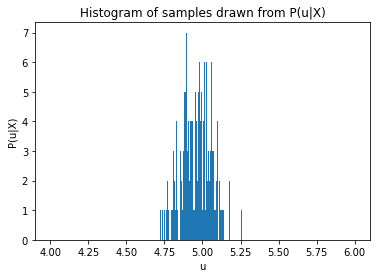
\includegraphics[width=0.5\linewidth]{image/q6/partc.png}
    \caption{Histogram of simulated values in Q6 Part c}
    \label{q6_simulation}
\end{figure}

\subsubsection*{Part d}

Here is the analytical solution. First we calculate $F(z)$ and then $f(z) = F'(z)$.

\begin{align*}
    F(z) & =  \mathbb{P} (e^X \leq z) \\
    & = \mathbb{P} (X \leq \log z) \\
    & = \mathbb{P} \left( \frac{X - \mu}{\sigma} \leq \frac{\log z - \mu}{\sigma} \right) \\
    & = \mathbb{P} (Z \leq \log z - \mu) \\
    & = \Phi(\log z - \mu)
\end{align*}

In the above calculations, $\Phi$ is the CDF of a standard normal distribution. To find $f(z)$ we use
$F(z)$.

\begin{align*}
    f(z) & = F'_Y(z) \\
    & = \frac{\partial}{\partial z} \Phi(\log z - \mu) \\
    & = \phi(\log z - \mu) / z
\end{align*}

Where $\phi = \Phi'$ is the PDF of a standard normal function.

\autoref{eu_density} shows the $\theta=e^\mu$ posterior density analytically and by simulation. Analyltical solution
discussed above but for the simulation we use data sampling and calculating the value for $e^\mu$.

\begin{figure}[h]
    \centering
    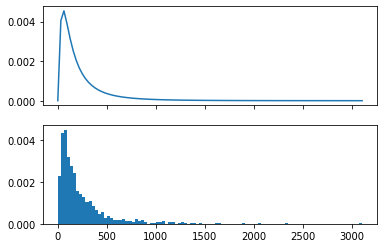
\includegraphics[width=0.5\linewidth]{image/q6/eu.png}
    \caption{Posterior density for $e^\mu$, analytically and by simulation}
    \label{eu_density}
\end{figure}

\subsubsection*{Part e}

We use simulation to calculate the value of confidence intervals. For $93\%$ posterior confidence interval
we have the range $(84.72, 833.64)$ and for $97\%$ we have the range $(16.06, 1238.79)$. As you can see the
interval for $97\%$ confidence interval is larger so be sure of the interval correctness.

\subsection*{Question Seven}

Assuming the number of deaths be $X \sim Bio(n, \theta)$, where $n=1919$.
We have a measurement for $X$, and we want to test the null hypothesis:

$$H_0:\theta=\frac{1}{2} \hspace{0.5cm} vs. \hspace{0.4cm} H_1:\theta \neq \frac{1}{2}$$

The best estimate for value of $\theta$ is caluclated by the formula $\frac{X}{n}=\frac{922}{1919}$ and the
standard deviation $\sqrt{\frac{\hat{\theta}(1-\hat{\theta})}{n}} = 0.01$. Hence the wald statistics is
$W = \frac{\hat{\theta} - \theta}{\hat{se}}=-1.71$. Comparing the $|W|$ with $z_{0.025}=1.95$ says we can't
reject $H_0$. Considering the p-value $8.7$\% there is a weak evidence against the null hypothesis.

\subsection*{Question Eight}

By repeating the Wald test for $1M$ times and counting number of rejection, we found out that
the false rejection ratio is $0.0512$ which is very close to $0.05$. Repeating the experiment results
in different raios but interestingly all of the experiments report values which are more than $0.05$.
Because of the confidence concept behind $\alpha$, it's interesting to have false ratio more than $\alpha$.

\end{document}